
%%%%%%%%%%%%%%%%%%%%%%% file typeinst.tex %%%%%%%%%%%%%%%%%%%%%%%%%
%5
% This is the LaTeX source for the instructions to authors using
% the LaTeX document class 'llncs.cls' for contributions to
% the Lecture Notes in Computer Sciences series.
% http://www.springer.com/lncs       Springer Heidelberg 2006/05/04
%
% It may be used as a template for your own input - copy it
% to a new file with a new name and use it as the basis
% for your article.
%
% NB: the document class 'llncs' has its own and detailed documentation, see
% ftp://ftp.springer.de/data/pubftp/pub/tex/latex/llncs/latex2e/llncsdoc.pdf
%
%%%%%%%%%%%%%%%%%%%%%%%%%%%%%%%%%%%%%%%%%%%%%%%%%%%%%%%%%%%%%%%%%%%


\documentclass[runningheads,a4paper]{llncs}

\usepackage[latin1]{inputenc}
\usepackage{graphicx,color,url}
\usepackage[dvips]{epsfig}
\usepackage{verbatim}
\usepackage{tikz}
\usetikzlibrary{external}
\usetikzlibrary{shapes,arrows}
\usetikzlibrary{calc,patterns,snakes,decorations.pathmorphing,decorations.markings}
\usetikzlibrary{positioning}

\tikzexternalize[mode=list and make]

\tikzset{
    png export/.style={
        % First we call ImageMagick; change settings to requirements
        external/system call/.add={}{; convert -density 300 -transparent white "\image.pdf" "\image.png"},
        % Now we force the PNG figure to be used instead of the PDF
        /pgf/images/external info,
        /pgf/images/include external/.code={
            \includegraphics[width=\pgfexternalwidth,height=\pgfexternalheight]{##1.png}
        },
      }
  }
  
\newcommand{\keywords}[1]{\par\addvspace\baselineskip
\noindent\keywordname\enspace\ignorespaces#1}


\providecommand{\tabularnewline}{\\}





\usepackage{amssymb}
\setcounter{tocdepth}{3}
\usepackage{graphicx}

\usepackage{url}
\urldef{\mailsa}\path|salemohammed@gmail.com|
\urldef{\mailsb}\path|amorag@geneura.ugr.es, jjmerelo@gmail.com|
\urldef{\mailsc}\path| fergunet@gmail.com|
\newcommand{\keywords}[1]{\par\addvspace\baselineskip
	\noindent\keywordname\enspace\ignorespaces#1}

\begin{document}
		
	% first the title is needed
	\title{Driving in TORCS using modular fuzzy controllers}
	
	
	%\titlerunning{Driving in TORCS using modular fuzzy controllers}
	
	
	
	
	\author{Mohammed Salem* \inst{1} \and Antonio Miguel Mora \inst{2}\and Juan Julian Merelo \inst{2} \and Pablo Garc\'ia-S\'anchez \inst{3}}
	
	
	
	%\authorrunning{M. Salem et al}
	% (feature abused for this document to repeat the title also on left hand pages)
	
	% the affiliations are given next; don't give your e-mail address
	% unless you accept that it will be published
	\institute{University of Mascara, Algeria\\
		\mailsa\\
		Department of Architecture and Computer Technology
		University of Granada, Spain\\
		\mailsb\\
		Universiy of C\'adiz, Spain
		\\
		\mailsc\\
	}
	
	%
	% NB: a more complex sample for affiliations and the mapping to the
	% corresponding authors can be found in the file "llncs.dem"
	% (search for the string "\mainmatter" where a contribution starts).
	% "llncs.dem" accompanies the document class "llncs.cls".
	%
	
	\toctitle{Driving in TORCS using modular fuzzy controllers}
	\tocauthor{}
	\maketitle
	\begin{abstract}
		
		When driving a car it is essential to take into account all possible
		factors; even more so when, like in the TORCS simulated race game, the
		objective is not only to avoid collisions, but also to win the race
		within a limited budget. In this paper, we present the design of an autonomous
		driver for racing car in a simulated race. Unlike previous controllers, that only used fuzzy logic approaches for either acceleration or steering, the proposed driver uses simultaneously two fuzzy controllers for steering and computing the target speed of the car at every moment of the race. They use the track border sensors as inputs and besides, for enhanced safety, it has also taken into account the relative position of the other competitors.
		The proposed fuzzy driver is evaluated in practise and timed races
		giving good results across a wide variety of racing tracks, mainly
		those that have many turning points.  
		
		\keywords{Videogames, Fuzzy Controller, TORCS, Steering control, Speed computation}
	\end{abstract}
	
	%
	%%%%%%%%%%%%%%%%%%%%%%%%%%%%%%%   INTRODUCTION   %%%%%%%%%%%%%%%%%%%%%%%%%%%%%%%
	%
	\section{Introduction}
	\label{sec:intro}
	
	The Open Racing Car Simulator (TORCS) \cite{WebTORCS} is a
	three-dimensional racing video game created by Eric Espi\'e and
	Christophe Guionneau, whose objective  is to be used as a
	framework to develop and test Artificial Intelligence (AI) models for
	autonomous drivers, named \textit{controllers} or bots. It is
	one of the most popular car racing simulators among the scientific
	community, and due to its open-source philosophy, there are
	several designers and programmers constantly improving it
	\cite{manualTORCS}. 
	
	
	Even if it does not have the graphic quality of commercial games, it
	presents several advantages for academic purposes, such as
	\cite{manualTORCS}: 
	
	\begin{itemize}
		\item  Its complexity lies between an advanced simulator, like recent commercial
		car racing games, and a fully customisable environment,
		like the ones typically used by computational
		intelligence researchers for benchmark purposes.
		\item  It features a sophisticated physics engine  that
		includes aerodynamics,
		fuel consumption, traction, as well as a 3D graphics
		engine for the visualization of the races.
		\item  It was not conceived as a free alternative to commercial
		racing games, but it was specifically devised to make it
		as easy as possible to develop and test your own controller. 
		In fact, controllers are implemented as separated software pieces with a 		 
		modular architecture, so it is easy to develop a new one and to plug 
		it into the game.
	\end{itemize}
	
	Even in simulation mode, driving a car with a bot as a human would do
	is a hard task, because the agent has to control several actions such
	as the steer, gear and brake/acceleration using the data related to
	the car and its environment (detected by means of sensors). 
	
	Hence, Computational Intelligence (CI) methods are interesting to be applied to the problem of implementing a car controller in TORCS \cite{Quadflieg_LearningTrack,CardamoneImitation09,MunozHumanLike10,Cardamone_Online_NN}. Among these techniques, Fuzzy logic \cite{abraham2001} with its adaptation and ability of imitating the human behaviour, is an interesting tool to design these drivers. It could be integrated in any controller module (steering, gear change, acceleration and brake, stuck) to give a human-like `appeal' to the bot driver \cite{CarRacing_Pelta09,torcs2012}.  
	
	In each simulation tick, the autonomous driver must make a decision,
	for instance, to direct the car (steer) on the track and select a
	target speed. This problem is much harder when the car is near to a
	curve where it has to choose a compromise between going faster and
	avoiding the car slips and goes out of the track. The overall idea is
	to move the car towards the farthest track border to avoid prematurely
	breaking. 
	
	This complex problem could be solved by means of Fuzzy Logic, due to
	its adaptive control and ability to deal with noise (in sensors
	\cite{manualTORCS}) and uncertainty (non-deterministic opponents'
	decisions in the race). Indeed, several researchers have taken advantage of this technique to design TORCS controllers, for example \cite{CarRacing_Pelta09,PerezEvolvingFuzzy09,torcs2012}. 
	% Antonio - TODO: poner más citas de controladores difusos en TORCS
	All the existing works used a specific fuzzy module with a concrete objective inside the controller's operation, such as computing the optimal acceleration, turning angle, or speed at every moment.
	
	However, this work presents a novel fuzzy-based controller, which implements two modular sub-controllers, each of them devoted to infer a specific target, namely: maximum speed and optimal steering for the car at every simulation tick.
	They consider the track sensors, to find the farthest border; and the opponents' position in the race, for collision avoidance and overtaking. 
	
	%The rest of this paper is organized as follows:
	%The next section presents the state of the art and related works, and comments their differences with regard to this study, along with its contribution to advance in this research line. TORCS simulator is described in Section \ref{sec:torcs}.
	%The proposed fuzzy controller (and its sub-controllers) is detailed in Section \ref{sec:fuzzy_controller}, whereas it is tested in `real' (simulated) races in Section \ref{sec:results}. Obtained results are analyzed and compared 
	%with other controllers are given in the same section. Finally, the conclusions and future lines of work are included in Section \ref{sec:conclusions}.
	
	
	%%%%%%%%%%%%%%%%%%%%%%%%%%%%%%  STATE OF THE ART  %%%%%%%%%%%%%%%%%%%%%%%%%%%%%%
	\section{Background and State of the Art}
	\label{sec:soa}
	
	In the last years, several researchers have focused on driving a racing car using computational intelligence techniques. 
	%
	%
	%TORCS + NN
	Among them, Artificial Neural Networks (ANN) have been one of the most prolific techniques successfully applied to this problem. For instance, using supervised methods it is possible to create controllers by the imitation of an existing bot \cite{CardamoneImitation09}. However, their performance decreases if they drive on circuits not previously used for training. In those cases, some authors have proposed automatic on-line (during the game) learning approaches, such as Quadflieg et al. \cite{Quadflieg_LearningTrack}, who implemented a recognition system based on a simple classifier to identify the part of the track where the car is; or Cardamone et al. \cite{Cardamone_Online_NN}, that proposed a neuroevolutionary method to adapt a controller to a new (unknown) track.
	
	Human data can also be used for training ANNs, or for example, to model a human-like controller \cite{MunozHumanLike10}. Although several scripts can be used to avoid noise, the problem to create a human-like driver is difficult, and again, their performance in circuits not known will be reduced, so a learning approach should be applied.
	
	%EA (con y sin TORCS)
	These models can be improved using meta-optimization techniques, such as Evolutionary Algorithms (EAs). These have been applied to `refine' the parameters \cite{ButzCMAES09} considered in the different methods (being them hand-coded or not), or to improve the structure/architecture of the models \cite{evol}. Thus, this can optimize the controllers' behavioural modules, and yield bots that might even win competitions \cite{ButzCMAES09,torcs2012}. EAs can also been used online during the game, to adapt a controller to the player skills \cite{TanOnline08,Cardamone_Online_NN}. Other approaches try to generate the source code of the controller from scratch using Genetic Programming \cite{AgapitosGP07}, although in the same evaluation time these approaches normally behave worse than standard ANN-based controllers. In these cases, higher population sizes might aid to outperform the latter.
	
	%FUZZY
	Another prolific technique has been Fuzzy Logic (FL), which has been widely used since the year 2008. For instance, Fujii et al. in \cite{Fujii2008} examined the performance of fuzzy rule-based systems for high-level decision making in a controller, along with the effect and influence of sensory information.
	In \cite{CarRacing_Pelta09}, a fuzzy controller was designed to obtain the target position for the car, whereas the steering was computed using a crisp formula. This work and its improvement \cite{torcs2012} have some common points with our proposal, as the controller is pretty similar, however, in this work two different specialized fuzzy modules have been implemented instead of just one.
	
	Some approaches are based on context-dependant hybrid fuzzy-sets, avoiding training and dealing with input variables \cite{ThangG08}. These authors claim that using Machine Learning techniques and fuzzy approaches may reduce the  training time. Although their approaches were applied to a different simulation environment, not to TORCS.
	
	%FUZZY + EAs
	EAs have been also used to optimize the fuzzy set parameters, although the maximum values of the sets may not be achieved following this approach \cite{PerezEvolvingFuzzy09}. In that work, the authors obtain improved fuzzy models to infer the acceleration and turning angle, but they are not specialized as the proposed here.
	
	In \cite{Guadarrama2008}, a fuzzy rule-based car controller for Car Racing Competition was built and tuned with co-evolutionary genetic algorithms. Indeed, two fuzzy controllers were designed: the first one to compute the acceleration using the velocity and distance and the second one to get the turning angle. But their approach was applied to a simpler simulator than TORCS.
	
	In this paper, we go a step further in the state of the art of TORCS fuzzy controllers, proposing a bot with modular or specialized fuzzy sub-modules for inferring on-line the target speed and the optimal steering at every point of the race. 
	
	
	
	%%%%%%%%%%%%%%%%%%%%%%%%%%%%  PROBLEM DESCRIPTION  %%%%%%%%%%%%%%%%%%%%%%%%%%%%
	\section{Problem Description: TORCS}
	\label{sec:torcs}
	
	The Open Racing Car Simulator (TORCS)\cite{WebTORCS} is a standalone application mainly designed as a framework or testbed for bots/controllers, which are built as separate modules loaded into the main memory when a race takes place \cite{Torcs3}, so they are quite independent fro the game engine itself.
	The main features of the architecture of TORCS are \cite{manualTORCS}: 
	
	\begin{itemize}
		\item TORCS is a client-server application, where the bots are run as external processes connected to the server through UDP connections.
		\item The simulation is achieved in real time with 20 ms per game tick. So, the server sends the values of the sensors to every controller and waits 10 ms (real time) to receive an action to conduct from the bot.
		If there is not a new action, the simulation continues and the last action is repeated.
		\item The TORCS software makes a physical separation between the driver code and the simulator itself. Hence, it defines an abstract layer that gives complete freedom of choice of the programming language used to implement the bots, and just gives access to some information.
	\end{itemize}
	
	There are several competitions which use TORCS as a base. During a competition, the bot perceives the race environment by means of a number of sensors, that provide information such as the status of the car, the status of the race, opponents' positions and track borders \cite{manualTORCS,torcs2}.
	Table \ref{t1} presents a complete list of available sensors with a description of each one.
	
	\begin{table}[ht!]
		{\scriptsize
			{\centering
				\begin{tabular}{|p{2cm}|p{3cm}|p{3 cm}|p{3 cm}|}
					\hline
					{\textbf{Sensor} }&
					{\textbf{Name} }&
					{\textbf{Range} (unit)} &  
					{\textbf{Data type}}\\ 
					\hline
					1 & angle & [-$\pi$,+$\pi$ ] & Double\\ 
					\hline
					2 & curLapTime & [0,+$\infty$] (s)	& Double\\ 
					\hline 
					3 & damage & [0,+$\infty$)(point)& Double\\ 
					\hline 
					4 & distFromStart & [0,+$\infty$) (m)& Double \\ 
					\hline 
					5 & distRaced &[0,+$\infty$) (m)& Double\\
					\hline 
					
					6 & focus & [0,200] (m)& Double\\
					\hline 
					
					7 & fuel & [0,+$\infty$) (l)& Double\\
					
					\hline
					8 & gear & \{-1,0,1,.. 6\}g& Integer \\
					
					\hline
					9 & lastLapTime &[0,+1] (s) & Double \\
					
					\hline
					10 & opponents &[0,200] (m)& Double \\
					
					\hline
					10 & racePos & \{1,2,...,N\} & Double \\
					\hline
					11 & rpm    & [0,+$\infty$) (rpm)   & Double \\
					\hline  
					13 & speedX & (-$\infty$,+$\infty$) (km/h) & Double\\
					\hline  
					14 & speedY &(-$\infty$,+$\infty$) (km/h)  & Double\\
					\hline 
					15 & speedZ & (-$\infty$,+$\infty$) (km/h) & Double \\
					
					\hline
					16 & track &  [0,200 ] & Double\\ 
					\hline
					17 & trackPos & (-$\infty$,+$\infty$) & Double\\
					
					\hline
					
					18 & wheelSpinVel  & [0,+$\infty$) (rad/s) & Double\\
					
					\hline
					19 & z &  (-$\infty$,+$\infty$) (m) & Double\\
					
					\hline
					
				\end{tabular}
			}
		}
		\caption{Description of available sensors in TORCS \cite{Torcs3}.}
		\label{t1}
	\end{table}
	
	Every TORCS driver bot is controlled by means of a set of actuators: the steering wheel `Steer', the accelerator `accel', the brake pedal and the gearbox. In addition, a meta-action is available to request a restart of the race to the server. Table \ref{tab2} details the available actions/actuators and their representation.
	
	\begin{table}[ht!]
		{\scriptsize
			{\centering
				\begin{tabular}{|p{3cm}|p{3 cm}|p{3 cm}|}
					\hline
					
					{\textbf{Action} }&
					{\textbf{Range} (unit)} &  
					{\textbf{Data type}}\\ 
					\hline
					Acceleration & [0,+1] & Double\\ 
					\hline
					Brake & [0,+1]	& Double\\
					\hline
					Gear & -1..0..+6	& Double\\
					\hline
					Steer & [-1,+1]	& Double\\
					\hline
					Clutch & [-1,+1]	& Double\\
					\hline
				\end{tabular}
			}
		}
		\caption{TORCS Actuators \cite{torcs2012}.}
		\label{tab2}
	\end{table}
	
	Hence, a controller is a program, which run inside TORCS, that automatically drives a car. It gets as input information about the current state of the car and its situation on the track. These collected data are used to compute actions to do in the next simulation tick; like steer, gear changes, acceleration or brake and clutch. A client may request a restart of the race by sending a special action on the server: Restart or shutdown \cite{manualTORCS}.
	
	The basic architecture of a controller consists of five simple modules (see Figure \ref{archi}), which are continuously working during a race. 
	
	\begin{figure}
		
		\centering
		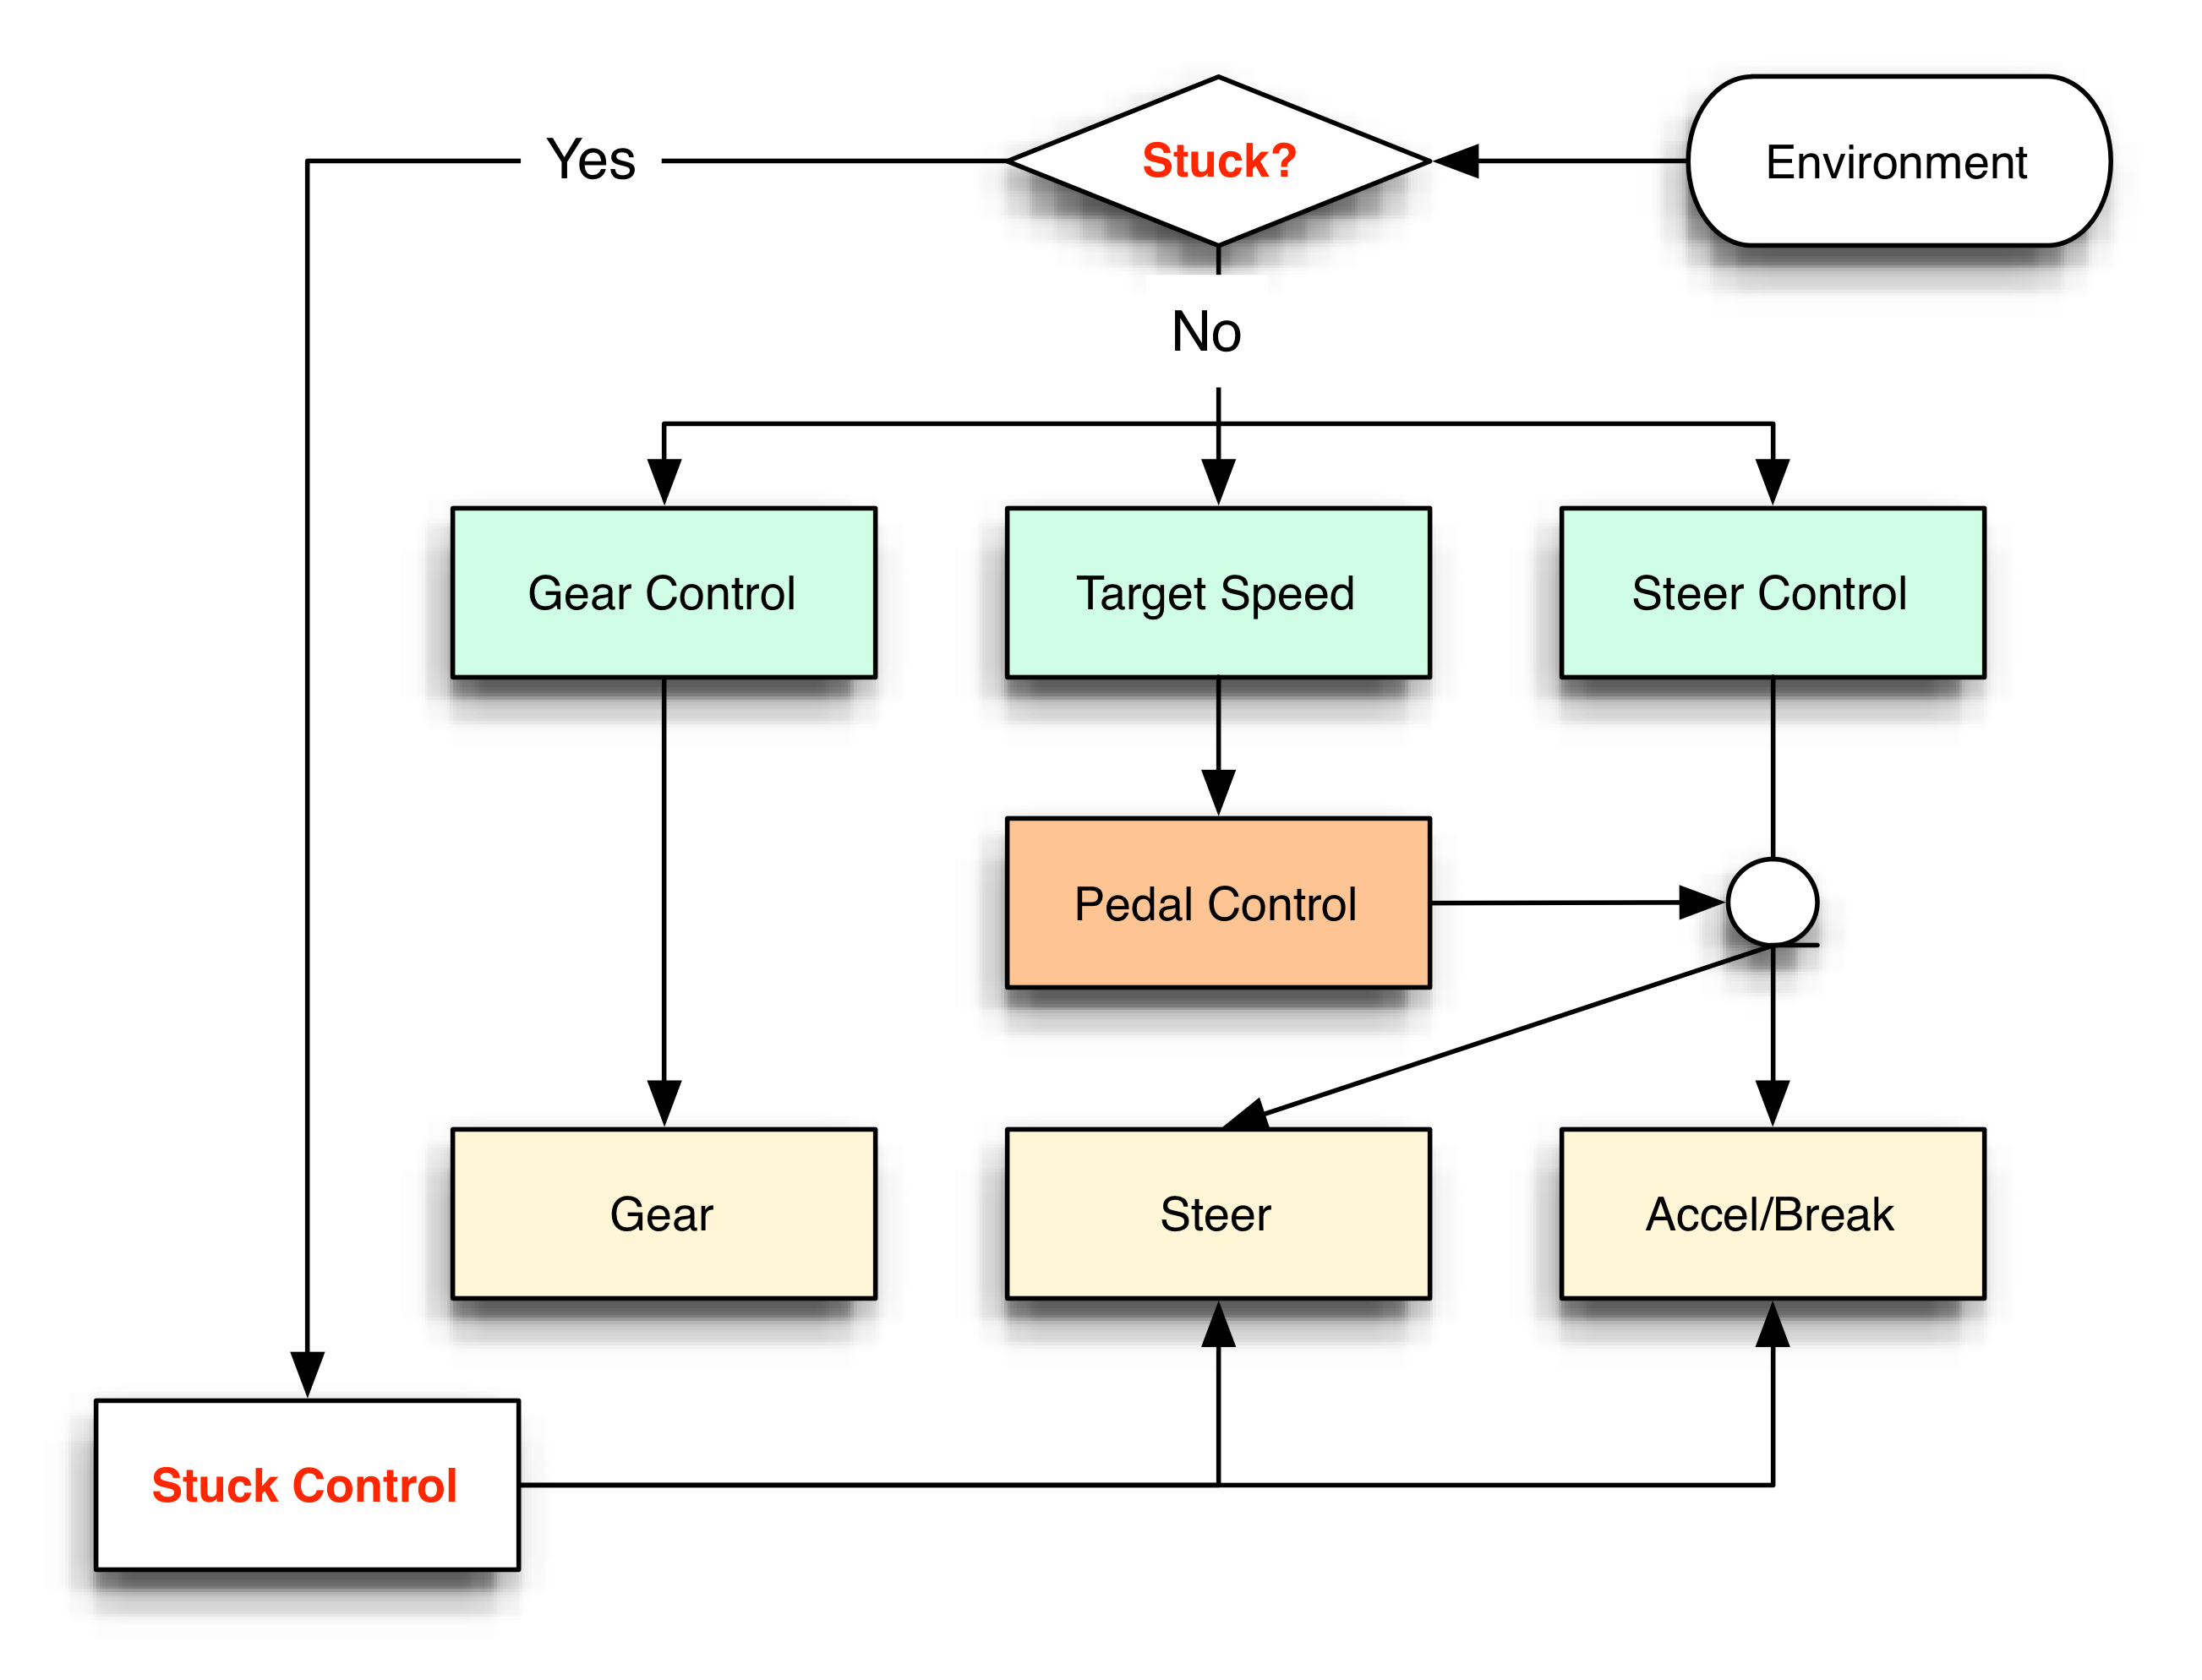
\includegraphics[width=0.8\textwidth]{fig/archicontrole-new.png}
		\begin{minipage}{10cm}
			\centering
			\caption{\footnotesize Basic architecture of a controller.}
			\label{archi}
		\end{minipage} 	
	\end{figure}
	
	TORCS comes with a simple example driver often used to validate new
	designed controllers \cite{CarRacing_Pelta09,torcs2}. It presents very basic
	functions for controlling the race car to give developers an idea of
	what the controller should look like. It includes simple functions to
	control the speed, steering angle and speed without dealing with
	opponents. We have used it as a baseline for comparison, as we will
	see later on.
	% Antonio - lo quito para ahorrar espacio
	% Lo vuelvo a poner porque sobra especio. 
	
	
	%%%%%%%%%%%%%%%%%%%%%%%%%%%  FUZZY CONTROLLER  %%%%%%%%%%%%%%%%%%%%%%%%%%%%
	%
	\section{Proposed Fuzzy Controller}
	\label{sec:fuzzy_controller}
	
	The proposed controller has the same modular architecture as the simple driver, and has some common functions of this approach. 
	However, the target speed and steering angle are computed by means of two modular and specialised fuzzy controllers, which consider five position sensors.
	
	In the following sections, each sub-controller is described.
	
	%-----------------------------------------------
	
	\subsection{Fuzzy target speed sub-controller}
	
	The first proposed fuzzy sub-controller aims to estimate the optimal target speed of the car, both in straight parts and curves of the track, taking into account two criteria: moving as faster as possible and secure the car. This estimation is based on fuzzy rules, so two general cases are considered, following the simple driver approach:
	
	\begin{itemize}
		\item If the car is in a straight line, the target speed will take a maximum value (\textit{maxSpeed} km/h).
		\item If it is close to a curve, the controller will decrease the current speed to a value included in the interval \textit{[minSpeed; maxSpeed]} km/h.
	\end{itemize}
	
	Thus, in case the car is out of the track or near a curve, the brake system is activated, and ABS (Anti-Block System) and TCL (Traction Control Limit) will be loaded to avoid the car skidding. The obtained target speed will be used for computing the value of acceleration, following - as the simple driver do - the expression:
	
	\begin{equation}	
	Gas(speed-Target_{speed})=-1+\frac{2}{1+e^{speed-Target_{speed}}}	
	\end{equation}
	
	\textit{Gas} function refers to acceleration, \textit{speed} is the current speed of the car.
	
	This fuzzy controller has three input values and one output: the target speed (see Figure \ref{fig:AD}).
	
	\begin{figure}
		\begin{center}
			
			\begin{tikzpicture}[box/.style={draw, fill=white!20,rounded corners,align=center,minimum height=3em, minimum width=5em},thick,->,>= latex]
			
			\node[box] (a0) {Fuzzy controller};
			\node[left=of a0.160,font=\bfseries] (aux01) {$Front$};
			\node[left=of a0.175,font=\bfseries] (aux02) {$M5$};
			\node[left=of a0.195,font=\bfseries] (aux03) {$M10 $};
			\node[right=of a0,font=\bfseries] (c0) {$Target_{speed}$};
			\draw[thick,->,>= latex] (aux01) -- (a0.160);
			\draw[thick,->,>= latex] (aux02) -- (a0.175);
			\draw[thick,->,>= latex] (aux03) -- (a0.195);
			\draw[thick,->,>= latex] (a0) -- (c0);
			\node[box,below=of a0] (b) {Inference};
			
			\node[box, left=of b] (a) {Fuzzification};
			
			
			\node[box,right=of b] (b1) {Defuzzification};
			
			
			\draw[thick,->,>= latex] (a) -- (b);
			\draw[thick,->,>= latex] (b) -- (b1);
			
			
			
			\draw[thick,->,>= latex] (a0.south west) -- (a.north west);
			\draw[thick,->,>= latex] (a0.south east) -- (b1.north east);
			
			
			\end{tikzpicture}
			
			%\includegraphics [width=10cm,height=4cm]{figures/c2/sif}
		\end{center}
		\caption{Fuzzy controller of target speed.}     % width is 8.4 cm.
		\label{fig:AD}
	\end{figure}
	%
	The controller presented in that figure is a Mamdani-based fuzzy system \cite{iancu2012} with trapezoidal Membership Functions (MF) for input variables, because it avoids sudden changes in input values. It considers three values among the 19 track sensors (see Figure \ref{fig34}):
	
	\begin{itemize}
		\item Front = Track[9]: the front distance between the car and the border of the track (angle 0º).
		\item M5 = max (Track[8], Track[10]): the max distance to the track limits in an angle of +5º and -5º with respect to Front.
		\item M10 = max (Track[7], Track[11]): the max distance to the border in an angle of +10º and -10º.
	\end{itemize}
	
	The set of sensors was chosen considering those used in previous works \cite{torcs2012}, but refining it after an exhaustive systematic experimentation phase. Thus, the final set of sensors are those which yielded the best results in a wider amount of tracks.
	
	\begin{figure}[ht!]
		
		\centering
		\includegraphics[width=0.8\textwidth]{fig/sensor22-new.png}
		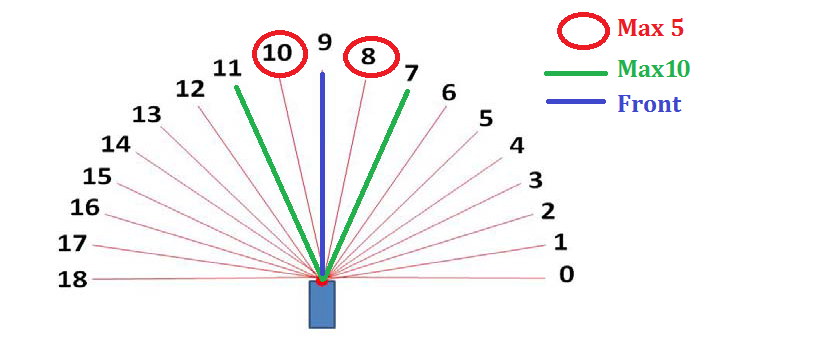
\includegraphics[width=0.7\textwidth]{fig/front.png}
		\begin{minipage}{10cm}
			\centering
			\caption{Inputs considered in the fuzzy sub-controllers.}
			\label{fig34}
		\end{minipage} 		
	\end{figure}
	
	Each input variable is represented by three membership functions: Low, Medium and High. The description of fuzzy inputs and output are represented in Table \ref{tab:flouevar}.
	
	\begin{table}
		\caption{Fuzzy variables description.}
		\label{tab:flouevar}
		\begin{tabular}{ |p{1.5cm}|p{2cm}|p{2cm}|p{2 cm}|p{1 cm}|p{1.5 cm}|p{1.5 cm}|}
			\hline
			{ \color{red} Variable }&
			{ \color{red} Range }&
			{ \color{red} Name}&  
			{ \color{red} MF } &
			{ \color{red} Low } &
			{ \color{red} Medium }&
			{ \color{red} High } 
			
			\\
			\hline
			\hline
			Input & [0-100] m & Front & trapezoidal & [0-50] & [20-80] & [60-100]
			\\
			\hline
			Input & [0-100] m & M5 & trapezoidal &[0-40] & [10-70] & [50-100] 
			\\
			\hline
			Input & [0-100] m  & M10 & trapezoidal & [0-30] & [20-60] & [50-100]
			\\
			\hline 
			Output & [0-200] m/s & TargetSpeed & singleton & / & / & /
			\\
			\hline 
		\end{tabular} 
	\end{table}
	
	The base of rules has been composed modelling the behaviour of a human expert driver, refining them also. Thus, this set is designed so that if the frontal distance is maximal, then the target speed should be the maximum. Its value should be lower when the frontal distance is shorter. 
	The fuzzy rules are listed below:
	
	\begin{itemize}
		\item IF Front is High THEN TargetSpeed is TS1
		\item IF Front is Medium THEN TargetSpeed is TS2
		\item IF Front is Low and M5 is High THEN TargetSpeed is TS3
		\item IF Front is Low and M5 is Medium THEN TargetSpeed is TS4
		\item IF Front is Low and M5 is Low and M10 is High THEN TargetSpeed is TS5
		\item IF Front is Low and M5 is Low and M10 is Medium THEN TargetSpeed is TS6
		\item IF Front is Low and M5 is Low and M10 is Low THEN TargetSpeed is TS7\\
		
		In addition, a crisp rule is added to rule base to obtain a maximum value of the target speed when the three input variables are as big as possible: 
		\item IF Front = MAXDISTSPEED or M5 = MAXDISTSPEED or M10 = MAXDISTSPEED THEN TargetSpeed = MAXSPEED		
	\end{itemize}
	
	MAXDISTSPEED is the a longest possible value for the track sensors, and MAXSPEED, which is related to the car's properties, is the maximal car speed. For example in the case of car-trb1 model, MAXSPEED=300.
	
	The output value is encoded by seven singletons TS1 to TS7, being respectively: 280, 240, 220, 180, 120, 60 and 30.
	
	%-----------------------------------------------
	
	\subsection{Fuzzy steering control sub-controller}	
	
	In addition to the speed sub-controller, another fuzzy approach has been applied to control the steering, estimating and determining the target position of the car. 
	
	The architecture of this sub-controller is similar to the one shown in Figure \ref{fig:AD}, but with the steering as output. The set of sensors considered are the same as in the speed case, described in Table \ref{tab:flouevar}.
	
	Then, if the car is in a straight line, it will set as target position half width of the race track (central position of the lane).	Whereas, if the car is near a right curve, it will approach the path leading to the right, with a space between the car and the border of the track to avoid the loss of control. The same approach is considered if the car is near a left curve.
	
	In order to detect the curves, the controller focuses on the sensor values (M10, M5, and Front). So, if the value on Front sensor is the longest, there is a straight road; whereas if the values of M5 and M10 with positive angles (+5 and +10) are the longest, there is right curve; and the other way round.
	
	The base of rules has been defined again modelling the behaviour of a human driver, so, for this controller is:
	
	\begin{itemize}		
		\item IF Front is High THEN steer is S1
		\item IF Front is Medium AND M10 is High THEN  steer is S2
		\item IF Front is Medium AND M10 is Medium AND M5 is Medium THEN steer is S2
		\item IF Front is Medium AND M10 is Medium AND M5 is Low THEN steer is S3
		\item IF Front is Low AND M10 is High THEN steer is S3
		\item IF Front is Low AND M10 is Medium AND M5 is Medium THEN steer is S4
		\item IF Front is Low AND M10 is Medium AND M5 is Low THEN steer is S4
	\end{itemize}	
	
	The values for S1 to S4 are respectively: 0, 0.25, 0.5, and 1.
	When M10=Track[7] we will take negative values of the steer (sterr=-steer).
	
	Once the controllers have been described, they will be tested and compared with the standard one y several races. The obtained results are presented in the following section.
	\section{Simulation Results}
	\label{sec:results}
	
	In this section we present all the experiments that we performed in order to measure the performance of our controller, called \textit{AD (Automatic Driver)}.
	We first, describe the methodology we have used and next, we present the experimental results of the implementation of the fuzzy driver, including opponents and using special criteria in each case.
	
	We have compared the proposed controller with the simple driver included in TORCS, so we have run every controller in several races in different tracks.
	We will start by an individual race by setting the laps number first and then a time trial race. The last test is a real test against TORCS drivers.
	
	% Antonio - describir un poco mejor los tests siguiendo también el comentario de JJ 
	% What do those tests imply? Are they like the
	% best way of doing that? The usual way? A
	% reference? Why 20 laps? - JJ
	
	% ------------------------------------------
	\subsection{Simulation settings}
	
	TORCS provides several tracks to choose which have been designed in order to test the performance of the controllers on different difficulty circuits and on different types of roads.
	In our case, we chose four circuits:
	
	\begin{itemize}
		\item Two road tracks: \textit{E-Road} and \textit{CG-Speedway Number1}, with a different associated difficulty, regarding the amount of curves and width of the road. Concretely \textit{E-Road} has been selected to check the performance of our controller on sinuous circuits, which are normally the hardest for other approaches. 
		\item A dirt road track: which increases the difficulty due to the lower grip of the dirty asphalt. \textit{Dirt1} has a good variety of curves, which also add an extra difficulty.
		\item An oval track: \textit{E-Track5} seems to be the most interesting, as it has curves in both directions.
	\end{itemize}
	
	Table \ref{Tabtrack} presents the properties and description of each selected track.
	
	\begin{table}
		
		\caption{Description of Selected tracks}
		\label{Tabtrack}
		\begin{tabular}{ |p{2cm}|p{1.9 cm}|p{2.2 cm}|p{2.1 cm}|p{2.2 cm}|}
			\hline
			\textbf{Track name}    & E-Track5
			& Dirt1 
			& E-Road
			& CG-Speedway Number1
			\\
			\hline
			\textbf{Shape}   
			& 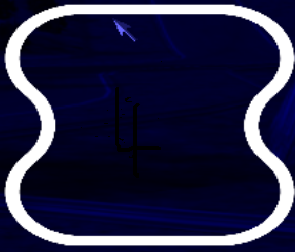
\includegraphics[scale=0.3]{fig/track4.png}
			& 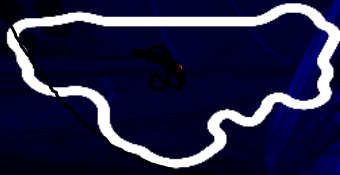
\includegraphics[scale=0.3]{fig/track2.png}
			%%	& %%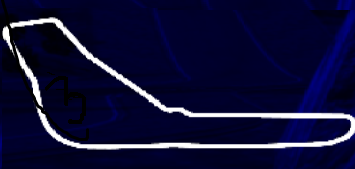
\includegraphics[scale=0.3]{fig/track3.png}
			& 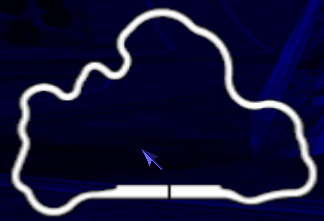
\includegraphics[scale=0.3]{fig/track5.png}
			& 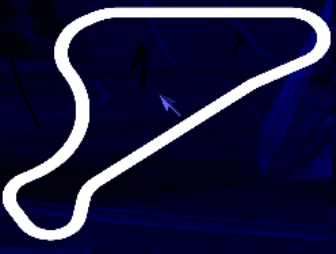
\includegraphics[scale=0.3]{fig/track1.png}
			
			\\
			\hline
			\textbf{Track Type}   
			& Oval
			& Dirty
			& Road
			& Road
			
			\\
			\hline
			
			\textbf{Length}   
			& 1621.73 m
			& 3260.43 m
			& 3260.43 m
			& 2057.56 m
			
			\\
			\hline
			\textbf{Width}   
			& 20.0 m
			& 16.0 m
			& 16.0 m
			& 15.0 m
			\\
			\hline
		\end{tabular} 
		
	\end{table}
	
	The aim of this selection is to test the value of AD in a wide set of situations, in order to check its potential as a global controller.
	
	
	% ----------------------------------------------
	
	\subsubsection{Cars settings.}
	
	The car considered is \textit{car1-tbr1} of SCR 1 Server, which is a NASCAR car part of the SCR Server team. It has a weight of 1150 KG, max fuel: 94 KG, length: 4.25m and width: 1.94m, with 300km/h as maximal speed.
	This is a fair car, i.e. not the fastest, but a quite fast. Anyway, the obtained results represents the quality of the controllers and could be extrapolated to any other car.
	
	% ----------------------------------------------
	
	\subsubsection{Controllers settings.}
	
	We have tested the different sub-controller features in a separated way, in order to see which one has the highest influence on the success or failure of
	AD. Thus, we have considered the following bots in the experiments:
	
	\begin{itemize}
		\item AD-SP: Fuzzy speed controller. 
		\item AD-SC: Fuzzy steering controller.
		\item AD-SSOP: Fuzzy speed and steering controller.
		This controller also takes the opponent into account. Thus, it considers the sensors that give the distance to the opponents from the car. If this distance is smaller than the distance to the border or the track (track sensor), it is used in the fuzzy rules.
		\item SD: Simple driver.
	\end{itemize}
	
	Since the speed controller is similar to previous approaches, it was expected to work properly. Hence, we have checked the basic version of our controller AD-SP and compared it with modified/improved versions, such as AD-SC and AD-SSOP.
	As stated before, SD has been taken as a baseline for comparisons.
	%Mohammed , si es verdad
	% Estoy con JJ en cuanto a que habría que haber probado todas las variantes (steering sólo, steering + oponente y speed + steering + oponente). ¿Hay alguna explicación para no haberlos incluido que podamos poner?
	
	% salem,  I validate the speed  controller and steer-speed one in alone race to  check the strength of the steer sub-controller  
	% Some reviewer could say why don't you take the opponent into
	% account with steering only or with target only, and also check only
	% fuzzy steering without controlling speed. You have to consider the
	% whole range of possibilities, and there are 6; you have considered
	% only 3. - JJ
	
	% ----------------------------------------------
	
	\subsection{Results of 20 laps practise race}
	
	We firstly test our controllers in the simplest case, a practise race without rivals. 
	We conducted a 20 laps race in the four tracks, aiming to check if the controllers are able to perform well in these `warm up' races.
	20 have been considered as it is the maximum number of laps a car can perform without doing a pit stop, because our controller is not prepared to plan and manage this event. 
	
	\begin{table}[h!]
		
		\caption{Results for 20 laps in practise races.}
		%	\label{resultat1}
		{\scriptsize
			\begin{tabular}{ |p{3.5cm}|p{2cm}|p{2cm}|p{2 cm}|p{2 cm}|}
				
				%	\multicolumn{5}{c}{\textbf{E-Track5}}\\
				\hline
				{ \color{blue}\textbf{E-Track5} }&
				{ \color{red}\textbf{SD}}&  
				{ \color{red} \textbf{AD-SP} } &
				{ \color{red} \textbf{AD-SC} } &
				{ \color{red} \textbf{AD-SSOP} }
				\\
				\hline
				Best Time & 01:05:15  & 01:21:24  &04:33:24 & 29:87 
				\\
				\hline
				Topspeed & 149  & 148 & 203 & 199 
				\\
				\hline
				Minspeed & 46 & 44 & 60 & 172 
				%		\\
				%		\hline 
				%		Lastlap	Time  & 01:05:17 & 01:31:36 & 01:02:55 & 30:07
				\\
				\hline 
				Best lap & 14 & 2 & 18 & 8 
				\\
				\hline
				Damage & 0 & 0 & 0 & 0 
				\\
				\hline 
				Fuel & 71.22 & 71.25 & 77.45 & 77.02 
				\\
				\hline
				%\multicolumn{5}{c}{\textbf{Dirt1}}\\	
				\hline
				{ \color{blue}\textbf{Dirt1} }&
				{ \color{red}\textbf{SD}}&  
				{ \color{red} \textbf{AD-SP} } &
				{ \color{red} \textbf{AD-SC} } &
				{ \color{red} \textbf{AD-SSOP} }
				\\
				\hline
				Best Time & 01:12:96 & 50:43  &02:23:12  & 35:51 \\
				\hline
				Topspeed & 132  & 126 & 136 & 139 
				\\
				\hline
				Minspeed &  21 & -52 & -43 & -54 
				%		\\
				%		\hline 
				%	
				%		Lastlap	Time  & 01:13:08  & 02:33:43 & 02:23:12 & 01:02:91 
				\\
				\hline 
				Best lap & 14 & 7 & 1 & 5 
				\\
				\hline
				Damage &  0 & 7438 & 905 & 9274 
				\\
				\hline 
				Fuel & 65.04 & 79.26 & 79.98 & 66.06 
				\\
				\hline
				%\multicolumn{5}{c}{\textbf{Forza}}\\	
				%%	\hline
				%	{ \color{blue}\textbf{Forza} }&
				%%		{ \color{red}\textbf{SD}}&  
				%		{ \color{red} \textbf{AD-SP} } &
				%		{ \color{red} \textbf{AD-SC} } &
				%		{ \color{red} \textbf{AD-SSOP} }
				%		\\
				%		\hline
				%		Best Time & 03:03:66  & 02:39:82 & 07:14:90  & 02:20:27 
				%		\\
				%		\hline
				%		Topspeed & 149 & 248 & 209 & 246 
				%		\\
				%		\hline
				%		Minspeed & 22  & -41 & -53 & 63 
				%		\\
				%		\hline 	
				%		Lastlap	Time  & 03:03:66 & 02:47:26 & 09:55:62 & 02:21:23
				%%		\\
				%		\hline 
				%		Best lap & 20 & 4 & 1 & 4 
				%		\\
				%		\hline
				%		Damage & 0 & 468 & 2269 & 0 
				%		\\
				%		\hline 
				%		Fuel & 62.61 & 71.88 & 60.55 & 60.55
				%		\\
				%		\hline
				%	\multicolumn{5}{c}{\textbf{E-Road}}\\	
				\hline
				{ \color{blue}\textbf{E-Road} }&
				{ \color{red}\textbf{SD}}&  
				{ \color{red} \textbf{AD-SP} } &
				{ \color{red} \textbf{AD-SC} } &
				{ \color{red} \textbf{AD-SSOP} }
				\\
				\hline
				Best Time & 02:44:93  & 02:11:39 & 04:33:59 & 01:25:66 
				\\
				\hline
				Topspeed & 149  & 202 & 203 & 207 
				\\
				\hline
				Minspeed & 24  & -58 & 32& -55 
				%		\\
				%		\hline 
				%		
				%		Lastlap	Time  & 02:45:08 & 03:00:20 & 04:51:53 & 01:27:38 
				\\
				\hline 
				Best lap & 3 & 3 & 17 & 3
				\\
				\hline
				Damage & 0 & 6056 & 7309 & 2239 
				\\
				\hline 
				Fuel & 62.11 & 78.25 & 79.25 &  55.22 
				
				\\
				\hline
				%\multicolumn{5}{c}{\textbf{CG-Speedway Number1}}\\	
				\hline
				{ \color{blue}\textbf{CG-Speedway Number1} }&
				{ \color{red}\textbf{SD}}&  
				{ \color{red} \textbf{AD-SP} } &
				{ \color{red} \textbf{AD-SC} } &
				{ \color{red} \textbf{AD-SSOP} }
				\\
				\hline
				Best Time & 01:25:00  & 01:12:99 & 01:12:23& 53:61 
				\\
				\hline
				Topspeed & 149  & 191& 194 & 178 
				\\
				\hline
				Minspeed & 49 & 57 & 32 & -51 
				%		\\
				%		\hline 
				%		
				%		Lastlap	Time  & 01:25:01 & 01:12:99& 01:29:65 & 01:46:47 
				\\
				\hline 
				Best lap & 12 & 20 & 2 & 2  
				\\
				\hline
				Damage & 0 & 0 & 0 &  114 
				\\
				\hline 
				Fuel & 66.66 & 62.58 & 73.38 & 60.65 
				\\
				\hline
			\end{tabular} 
		}
		\label{Result1r}
	\end{table}
	
	The table \ref{Result1r} shows that among the four drivers, the
	minimum time has been achieved by the AD-SSOP controller in each of the
	four tracks. This was due to the steering unit of the controller, which allows late braking, and thus, getting and maintaining a maximal speed (as it can be seen on the third  row of every table), along with following optimal paths to earn race time.
	
	The target position allows the car to safely adjust the required steering angle with the maximum speed so the controller AD-SSOP gave the best time. However, taking a smaller target angle required a greater distance to
	cover by the car which follows a less efficient trajectory. In addition, the
	number of times the car was off the road on Dirt1  was higher
	for AD-SSOP and thus, this controller gets a higher damage due to the collision with the outer walls of the track. 
	
	The simple SD driver finished the race without damage, while AD-SSOP was able to complete E-Track5  track safely and with damage for the others. The damage was also a little high for the AD-SP driver. 
	
	Regarding the Fuel consumption, it  depends on shocks rate and category of tracks, because it is required to accelerate more after a collision or depending on the grip, for instance.  
	
	AD-SC gets quite bad results, even in the comparison with the simple driver, so it means that the use of only the steering controller is not recommended, and it must be combined with any other. 
	
	The novel controllers seem to be robust in the sense that they obtain their best marks from their first laps, as a difference to the SD, which usually requires a higher amount of laps to improve its times.
	
	% ----------------------------------------------
	
	\subsection{Time trial race}
	
	In the second experiment, the race stopping criterion is set to 300s, so, after that time, the simulation stops. There are no opponents again.
	Once the race has ended, the distances covered by each controller are checked.
	
	The results are shown in Table \ref{resulta9} where it could be seen that the the AD-SSOP controller has yielded the best results in the oval and road tracks. However, in the dirty one, it was a disaster, since it was extremely damaged and TORCS simulator had to stop it. For this reason, the distance covered by this controller is the smallest. 
	
	This happened to the lack of grip in this kind of tracks and the damages which were caused by the crashes/collisions with the track border. 
	AD-SC also showed problems in the same circuit so this lead us to reinforce the fact the fuzzy steering control module is too much sensitive to the bad conditions of the road. This is a point of improvement that we will address in a close future.
	
	\begin{table} 
		
		\caption{Results of the controllers in 300 seconds time trial race.}
		\label{resulta9}
		{\scriptsize
			\begin{tabular}{ |p{3.5cm}|p{3cm}|p{3cm}|p{2.5cm}|}	
				%		\multicolumn{4}{c}{\textbf{E-Track5}}\\	
				\hline
				{ \color{blue}\textbf{E-Track5} }&
				{ \color{red}\textbf{Best Time Lap} }&
				{ \color{red} \textbf{Distance} } &
				{ \color{red} \textbf{Top speed} }
				\\
				\hline
				AD-SP &01:11:98  &4540.844&  155
				\\
				\hline
				AD-SC & 02:15:26 &8803.161& 155
				\\
				\hline 
				AD-SSOP & 29:30&32600&199 
				\\
				\hline 
				%		\multicolumn{4}{c}{\textbf{Dirt1}}\\			
				\hline
				{ \color{blue}\textbf{Dirt1} }&
				{ \color{red}\textbf{Best Time Lap} }&
				{ \color{red} \textbf{Distance} } &
				{ \color{red} \textbf{Top speed} }
				\\
				\hline
				AD-SP & 04:49:12 & 7825.032&126  
				\\
				\hline
				AD-SC & 03:45:02 &5202.99& 134
				\\
				\hline 
				AD-SSOP & 01:36:14 &4620.25& 153 
				\\
				\hline 
				%		\multicolumn{4}{c}{\textbf{Forza}}\\		
				%		\hline
				%		{ \color{blue}\textbf{Forza} }&
				%		{ \color{red}\textbf{Best Time Lap} }&
				%		{ \color{red} \textbf{Distance} } &
				%		{ \color{red} \textbf{Top speed} }
				%		\\
				%		\hline
				%		AD-SP & 02:49:12  & 17352.30  &  247
				%		\\
				%		\hline
				%		AD-SC & 02:49:12  & 17354.12 & %239
				%		\\
				%		\hline 
				%		AD-SSOP & 57:66 & 17355.20 & 203 
				% Antonio - ¿Está el valor de velocidad de AD-SSOP bien? Siempre ha sido el que más velocidad alcanza.
				%		\\
				%		\hline 
				%	\multicolumn{4}{c}{\textbf{E-Road}}\\	
				\hline
				{ \color{blue}\textbf{E-Road} }&
				{ \color{red}\textbf{Best Time Lap} }&
				{ \color{red} \textbf{Distance} } &
				{ \color{red} \textbf{Top speed} }
				\\
				\hline
				AD-SP & 03:62:33 & 11586.2 &  160
				\\
				\hline
				AD-SC & 02:41:41  & 11588 & 208 
				\\
				\hline 
				AD-SSOP & 01:15:16 & 23139 & 217
				\\
				\hline 
				%			\multicolumn{4}{c}{\textbf{CG-Speedway Number1}}\\
				\hline
				{ \color{blue}\textbf{CG-Speedway Number1} }&
				{ \color{red}\textbf{Best Time Lap} }&
				{ \color{red} \textbf{Distance} } &
				{ \color{red} \textbf{Top speed} }
				\\
				\hline
				AD-SP & 01:15:19 & 23136 &  195
				\\
				\hline
				AD-SC & 01:15:80 & 17352.2 & 193 
				\\
				\hline 
				AD-SSOP & 44:67& 28921.6 &206 
				\\
				\hline 
				
			\end{tabular}
		}
	\end{table}
	
	% ----------------------------------------------
	
	\subsection{Real race}
	
	Finally, a real race test has been conducted. Our main goal is to test the performance of our best controller, AD-SSOP, in a race, and answer the following questions: Could we have a perfect driving in a race with AD-SSOP only with the track borders and opponents' sensors? Can we win the race with AD-SSOP?
	
	In this context we tested this controller in 5 tracks against \textit{berniw, bt, damned, inferno} and \textit{tita} teams which are integrated TORCS controllers with different strategies and slightly modifications. Moreover, \textit{bt} controller comes with advanced machine learning methods \cite{oponnents2010}.
	
	% Antonio - creo que habría que explicar brevemente cada uno de ellos. ;D
	
	After the launch of every race, AD-SSOP against the 10 cars of each team for 20 laps in each track, we obtained the results presented in Table \ref{resultat31}.
	
	\begin{table}[ht!]
		\caption{Results of AD-SSOP in a real race.}
		\label{resultat31}
		{\scriptsize
			\begin{tabular}{ |p{2cm}|p{2cm}|p{2cm}|p{2 cm}|p{2 cm}|p{2 cm}|}
				\hline
				{ \color{blue}\textbf{E-Track5} }&
				{ \color{red}\textbf{Against berniw team }}&  
				{ \color{red} \textbf{Against bt team} } &
				{ \color{red} \textbf{Against damned team} } &
				{ \color{red} \textbf{Against inferno team} }&
				{ \color{red} \textbf{Against tita team} }
				\\
				\hline
				Ranking & 1/11 & 2/11   & 1/11 & 7/11& 4/11
				\\
				\hline
				Best time & 29:90 & 30:28   & 30:28 & 30:59& 30:53 
				\\
				\hline 
				Maxspeed & 198 & 198 &  198 & 199 & 198
				\\
				\hline
				
				Damage & 2267 & 7939 &  5888 & 5232& 8043
				\\
				\hline 
				\hline
				{ \color{blue}\textbf{Dirt1} }&
				{ \color{red}\textbf{Against berniw team }}&  
				{ \color{red} \textbf{Against bt team} } &
				{ \color{red} \textbf{Against damned team} } &
				{ \color{red} \textbf{Against inferno team} }&
				{ \color{red} \textbf{Against tita team} }
				\\
				\hline
				Ranking & 10/11 & 11/11 & 11/11 & 11/11 & 10/11
				\\
				\hline
				Best time& 05:11:45 & 05:07:79 & 05:39:33 & 05:27:96   & 05:37:16
				\\
				\hline 
				Maxspeed & 146 & 141 & 145 & 145 & 145\\
				\hline		
				Damage & 10017 & 6462 & 39 & 226& 5593\\
				
				\hline
				\hline
				%%	{ \color{blue}\textbf{Forza} }&
				%%	{ \color{red}\textbf{Against berniw team }}&  
				%%		{ \color{red} \textbf{Against bt team} } &
				%%		{ \color{red} \textbf{Against damned team} } &
				%%		{ \color{red} \textbf{Against inferno team} }&
				%%		{ \color{red} \textbf{Against tita team} }
				%%		\\
				%%		\hline
				%%		Ranking & 10/11  & 11/11 & 11/11 & 10/11& 10/11
				%%		\\
				%%		\hline
				%%		Best time & 01:57:58 & 01:45:30 & 02:03:00 & 02:04:00& 02:04:37
				%%		\\
				%%		\hline 
				%%		Maxspeed & 243  & 282 & 260 & 220& 217
				%%		\\
				%%		\hline
				
				%%		Damage & 2275 & 95 & 475 & 416 & 1185
				%%		\\
				
				%%		\hline 
				%%		\hline
				{ \color{blue}\textbf{E-Road} }&
				{ \color{red}\textbf{Against berniw team }}&  
				{ \color{red} \textbf{Against bt team} } &
				{ \color{red} \textbf{Against damned team} } &
				{ \color{red} \textbf{Against inferno team} }&
				{ \color{red} \textbf{Against tita team} }
				\\
				\hline
				Ranking & 2/11 & 2/11 & 8/11 & 7/11 & 10/11
				\\
				\hline 
				Best time& 01:21:29  & 01:29:92 & 01:39:54 & 01:27:27   & 01:48:18
				\\
				\hline 
				Maxspeed & 205 & 201 & 212 & 211 & 208
				\\
				\hline
				
				Damage & 9979 & 10362 & 4421 & 7685 & 5593
				\\
				
				\hline 
				\hline
				{ \color{blue}\textbf{CG-SpeedWay Number1} }&
				{ \color{red}\textbf{Against berniw team }}&  
				{ \color{red} \textbf{Against bt team} } &
				{ \color{red} \textbf{Against damned team} } &
				{ \color{red} \textbf{Against inferno team} }&
				{ \color{red} \textbf{Against tita team} }
				\\
				\hline
				Ranking & 2/11  & 4/11  & 1/11  & 5/11& 6/11
				\\
				\hline
				Best time & 46:16   & 48:56 & 47:23 & 46:06& 03:41:41
				\\
				\hline 
				Maxspeed & 205 & 202 & 199 & 200 & 198
				\\
				\hline		
				Damage &5533 & 3096 & 5093 & 5501& 4345		\\
				\hline 
				
				
			\end{tabular} 
		}
	\end{table}
	
	From Table \ref {resultat31}, we noticed that our controller has won the race in E-Track5 (oval track), and also got good positions against all the teams but inferno. This lead us to think that it is quite good for this type of circuit, due to the optimal trajectory in curves computed by means of the steering sub-controller, which also allows braking as late as possible.
	Furthermore, the target speed sub-controller allowed to go as fast as possible. In E-Road and CG-SpeedWay Number1 the results are also very competitive, except against the teams {\em inferno} and {\em tita}.
	
	The obtained damage happens because when our controller is in parallel with its opponent, close to it in a narrow track they shock between them.
	According to damage results, despite our controller can win the race on the E-track5 and CG-SpeedWay Number1, it had a higher crash rates in several cases. We observed also that in the majority of cases our car is very slow compared to the other cars in each team. 
	
	In the Dirt1 which has the difficulty of a lower grip, the drawbacks of the proposed controller had clearly affected the results.
	
	
	%%%%%%%%%%%%%%%%%%%%%%%%%%%%%  CONCLUSIONS  %%%%%%%%%%%%%%%%%%%%%%%%%%%%
	%
	\section{Conclusions and Future Work} 
	\label{sec:conclusions}
	
	In this work, a novel fuzzy driver for TORCS has been presented. It is based on two fuzzy sub-controllers, able to compute the target speed and the steering respectively. The aim of the proposed controller is to direct the car to the farthest side of the track in curves so to keep the target speed as high as possible. 
	
	This approach differs from others in the state of the art due to the combination of both sub-controllers, which is a novel variation.
	
	The designed controller has been evaluated in four circuits with different shapes and conditions and considering three different scenarios: a practise race, a time trial race, and a real race against tough opponents belonging to TORCS teams. Three different combinations of the fuzzy modules have been tested, namely one with the target speed computation (AD-SP), one with just steering control (AD-SC), and one with both of them plus the consideration of the opponents (AD-SSOP), when there exist.
	
	The obtained results have been very good in practise and time limit races, mainly for AD-SSOP. It has also behaved very well in the real races in one of the circuits (an oval one), ranked in the first positions. It has happened because the optimal trajectory computation conducted by the steering sub-controller, which allows late braking. However, this approach tends to receive too much damage, due to the crash with rivals or with the borders of the tracks, mainly when the road is not in optimal conditions, e.g. it is dirty.
	This is the main point of improvement that we will address in the close future.
	
	In addition, in future work we also aim to improve the controller to design a smarter racing car driver. This could be enhanced by tuning its parameters using an evolutionary algorithm or/and combine it with a learning tool (neural networks) to recognize the track parts and plan in advance.
	
	
	%%%%%%%%%%%%%%%%%%%%%%%%%%%%%%%%%%%%%%%%%%%%%%%%%%%%%%%%%%%%%%%%%%%%%%%
	
	\section*{Acknowledgements}
	
	This work has been supported in part by projects 
	EPHEMECH (TIN2014-56494-C4-3-P, Spanish Ministerio de Economía y Competitividad), 
	PROY-PP2015-06 (Plan Propio 2015 UGR), 
	PETRA (SPIP2014-01437, funded by Direcci\'on General de Tr\'afico),
	CEI2015-MP-V17 (awarded by CEI BioTIC Granada), and 
	PRY142/14 (funded by Fundaci\'on P\'ublica Andaluza Centro de Estudios Andaluces en la IX Convocatoria de Proyectos de Investigaci\'on).
	\bibliographystyle{splncs03}
	\bibliography{fuzzy_torcs}
	
	
	
	
	
	
\end{document}
